\documentclass[a4paper,11pt]{article}
\usepackage[english]{babel}
\usepackage[latin1]{inputenc}
\usepackage[dvips]{graphicx}
\usepackage{listings}
\usepackage{moreverb}
\usepackage{float}
\usepackage{fancyhdr}
\usepackage{algorithmic}
\usepackage{amsmath}
\usepackage{array}
\usepackage[final]{pdfpages}
\usepackage{url}
\usepackage{listings}


\textheight=21.0cm
\textwidth=15.1cm

\topmargin=-1.0cm
\headsep=0.7cm
\oddsidemargin=0.4cm
\evensidemargin=0.4cm

\footskip=1.0cm
\setcounter{secnumdepth}{3}

\fancyhf{}
\fancyhead[LE,RO]{\slshape \rightmark}
\fancyhead[LO,RE]{\slshape \leftmark}
\fancyfoot[C]{\thepage}

\begin{document}
\begin{titlepage}

%forside
\thispagestyle{empty}
\begin{center}        % sentrerer teksten
  \vspace{58mm}          % vertikalt mellomrom

\vspace{23mm}
  \Large
  \textbf{\\$ $\\$ $\\Project Sokoban} \\ $ $ \\
  \large
  \vspace{5mm}
  \textbf{by} \\$ $\\$ $\\ $ $ \\

  \vspace{5mm}
  %Forfatter
  \large
  \textbf{M�rten P�lsson} 8802030539 $<$mpals@kth.se$>$ \\
\textbf{Henrik Sohlberg} 8805080531 $<$hsoh@kth.se$>$ \\
\textbf{Simon �sterman} 8802050156 $<$simost@kth.se$>$ \\

 \vspace{25mm}
  \vspace{2mm}
	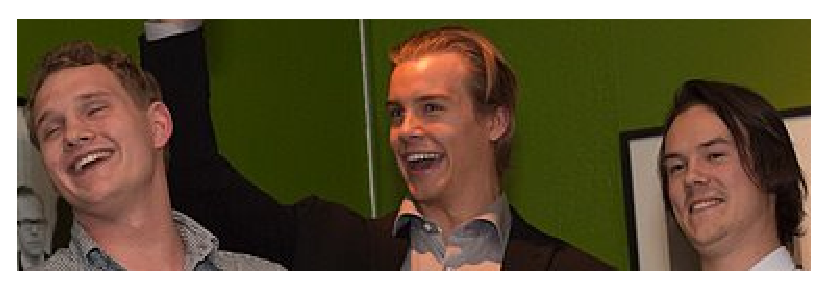
\includegraphics[scale=0.6]{2.eps}
	\emph{\\In order}\\ $ $ \\

 
  \vspace{5mm}
  \vspace{8mm}
  \vspace{0mm}
	\textbf{KTH Computer Science and Communication\\}
	\emph{DD2380 - ai12} \\
  \vspace{15mm}
 \vspace{30mm}

  \textsl{2012-10-10} \\
\end{center}

\end{titlepage}
\pagestyle{empty}
\clearpage
$ $
\clearpage

\abstract
Sokoban is a single-player game where your goal is to push boxes across a map and place them on specified goals. This report covers our implementation of an agent that aims to solve the game of sokoban. Our solution was a forward searching algorithm that used a prioritized queue while pruning away ''dead'' maps with deadlock detection. 
It did not however use any concrete ways of lessening the search area of the algorithm. This coupled with the huge branching factor of sokoban and the immense depth of its search tree meant that we could not solve more complex maps.\\\\\\

\newpage
\tableofcontents
\newpage
\pagestyle{fancy}
\setcounter{page}{1} % sets the current page number to 32 

\section{Introduction}
For this project we have programmed an agent that plays the game of sokoban. Sokoban is a single-player game where your goal is to push boxes across a map and place them on specified goals. The map consists of walls, boxes, goals and the player itself. To win a game of Sokoban, all of the boxes on the map have to be placed on a goal.\cite{1}
\section{Problem}
The problem for this project consists of creating an agent that will solve Sokoban boards in under 60 seconds and using less than 500 MB of memory. A solution to the board is to be provided as a string of letters where every letter represent a move made by the player. So ''RRDL'' means that the player moved: right, right, down and left before reaching a winning state. 
In the game of Sokoban, a box can only be pushed, thus to move a box the player will have to move to stand beside the opposite facing of the box from the direction he wants to push, and move onto the position that the box earlier occupied. 
The game is won when all the goals on the map are occupied by a box. This will henceforth be referred to as a \emph{winning} state. A state is simply a specific instance of the Sokoban map with the boxes, their positions and the position of the player itself. Thus every time you push a box, a new state is created.
\section{Approach}
\subsection{Design Approaches}
There are two basic approaches to solving sokoban. Either a forward searching algorithm where you evaluate possible new states from the players point of view. This means that the starting state is the board you are presented with at the beginning of the game. Each new state is created from pushing a box to a new position and adding that state to a queue.
The second is reverse searching. This kind of search begins with the possible winning states and all new states are calculated by pulling a box. This search ends when you have reached the starting state. 
These two search approaches can be combined to minimize the search area of the algorithm and thus reach a conclusion faster.

\subsection{Our Approach}
The Sokoban solver agent we created for this project is simple and straightforward. It uses a  forward searching algorithm with a breadth-first search with a prioritized queue (A* search) while pruning away dead states with both static and dynamic deadlock detection. 

Since our solution uses a forward-searching algorithm, the state we start with is the same as the board we get as input. A child-state is created by performing a push on one box in the current state. This is the only way a new state is created since the way the player moves between the pushes is uninteresting at the time and is therefore not saved in the new state. Before creating a new state we check so that the push is legal which for us means that it is not prevented by an obstacle or causing a deadlock. A new child-state is created if the push is legal, the state has not been visited before and if there are pushes available in it. The new child-state then gets evaluated and inserted into the prioritized queue according to the value assigned to it by the evaluation. The state with the highest value is inserted at the head of the queue so that we visit the most promising states first. 

The heuristics we use for the evaluation are based on the mobility of the boxes in the state, how many boxes are currently on a goal as well as the distance from the boxes to the closest goal. 

New child states are created and visited in this fashion until we reach a winning state. This state is then returned and all we have to do is to reconstruct the path the player took from the original state, as each (except the starting) state contains a pointer to its parent state. These pointers are followed from the winning state to the state we started in whilst creating a pointer in the opposite direction. Then we can easily create the solution string by just following the pointers from state to state until the end. The path of the player between the states is calculated by looking at the current state and the box-push that created the child-state (kept in the state-object) and then doing a breadth-first search between those positions on the board.   


In order to do all of the above efficiently, we hashed every state and removed some of the positions of the board which we could determine as deadlocks. 

We avoid repeated states by hashing every state before we add it to the queue and comparing it to already computed hashes. The hash function takes into consideration where the player and the boxes are located in a specific state. The initial deadlock detection functionality limits the number of cells boxes may be pushed onto, the hash function uses this information and creates a unique value for the possible cell number sequence 0-31, 32-63 and so forth. Each value is the size of an integer (32 bits) and each bit tells if there is a box on that position (a 1) or not (a 0). The least number of keys will be two (player and boxes concerning 32 number of cells) and will use a hashmap-in-a-hashmap data structure. 

Deadlock detection refers to finding spots on the sokoban playing board such that if a box is placed there, it will create a ''dead'' map. I.e it is impossible to push the aforementioned box to the goal from that location and thus impossible to win. 
These dead locations are calculated once at the start of the game since they will remain static throughout the entire search.
Dynamic deadlock detection refers to two boxes creating a deadlock together in a position that would not normally be considered a deadlock. This is done by finding boxes that are pushed next to another box along a wall, effectively locking them both in place since none of them can now be pushed in any direction.

\subsection{Pseudo code}
\begin{algorithmic}
\STATE Find the winning map
\STATE $currentState \leftarrow startMap$
	\WHILE{$newStates$}
		\STATE $currentState \leftarrow prioQueue.remove;$
		\FOR{$all$ $moves$ $in$ $currentState$} 
			\STATE $nextMap \leftarrow new Map(move)$
			\IF{$nextMap$ $is$ $winning$ $state$}
				\RETURN $nextMap$
			\ELSIF{$nextMap$ $has$ $moves$ $\&$ $!visited$}
			\STATE $prioQueue \leftarrow nextMap$
			\ENDIF
		\ENDFOR
	\ENDWHILE
\RETURN
\end{algorithmic}

\section{Results}
\begin{tabular}{ c | c}

\textbf{Solved maps} & \textbf{Reason for not solving} \\ \hline
$40/100$ & Time-out\\ \hline
\end{tabular} 

\section{Discussion}
While there are always several programming issues that can slow down an algorithm (such as inefficient use of variables etc), we will ignore these for the sake of briefness and concentrate on the larger implementation decisions taken in the creation of the solver.

Sokoban is a difficult problem since it has a huge branching-factor and generates an enormous search tree \cite{2}. This can be tackled in different ways. 
Our approach to this problem was by using a heuristic to evaluate each state and putting them in a priority queue. This gives the solver an incentive to search for winning states instead of just new states. Thus, hopefully minimizing the time spent evaluating states that are hopeless causes and making the search tree smaller or at least hopefully makes the solver search through a smaller part of the tree. 
How the evaluation helps the performance of the algorithm is obviously very dependent on the design of the board. In this way our heuristic can on some boards have hamstrung our solver and slowed it down.

While the heuristic can in some cases lessen the area of the search tree that we iterate through, it does nothing to actually make the search area smaller. This could have been done by complementing our forward search with a backward search which means that we would search backwards and forwards at the same time. When the two searches meet, they can then be appended to each other and a solution be produced. This would have made the search area smaller since instead of (worst case scenario) searching all possible permutations of the board until a winning state was found, two smaller searches will be performed. These smaller searches would theoretically meet before the entire search tree was iterated over and thus find a solution faster. 

Another small way to lessen the amount of states evaluated is by implementing tunnel detection. This refers to the fact that a tunnel can actually be considered traversed in a single push on a box since the moves in between are only interesting when printing the solution. This would remove all of the superfluous states in between and make the search shorter.
\newpage
\section{Conclusion}
Since we did not implement any concrete ways to lessen the amount of states that would have to be evaluated, and since the branching factor of sokoban is so big. It is not surprising that we could not solve more complex boards in the time allotted to us. 
\section{Reflection} 
When we started planning the project our idea was to create a simple and straightforward forward search algorithm with static deadlock detection. We did this because it was easy to implement and modify.
The work was split evenly between the group members and we discussed each stage of the program before we set to work. Henrik concentrated on our hash-algorithm, M�rten on deadlock detection and Simon worked with the utility functions such as finding the possible moves in a state. 

While working, we discovered that our approach was too slow by running the boards on the test server and timing out,  so we implemented a prioritized queue and heuristic. This was later complemented with dynamic deadlock-detection to further prune away dead states. 
When developing our heuristic we tried many different things. One thing we quickly learned to not weigh too heavily was mobility, i.e how many possible moves could be performed in each state. This was because many maps had goal locations that would lock the boxes in place and thus would weigh less than a losing state that had high mobility.
In the end  we ended up with a heuristic that uses Manhattan-Distance for evaluating how close the box is to a goal as well as a heavy emphasis on boxes on goals and a small weight on mobility.

If we would do this again we would try do find a better way of identifying repeated states. The implementation of our agent, for example, does not take advantage of the fact there are $n$ number of boxes but instead is determined by the number of cells boxes could stand on. Furthermore, we would implement a backward-search to complement our forward-search to limit the search area of our algorithm. This would make the algorithm faster and let us solve more boards. 
\newpage
\begin{thebibliography}{9}
\bibitem{1} Homework 1. [Homepage on the Internet]. [cited 10/10/12]. Available from: \url{http://dd2380.csc.kth.se/hw/hw1/assignment/}

\bibitem{2} Sokoban [Homepage on the Internet]. [cited 10/10/12]. Available from: \url{http://en.wikipedia.org/wiki/Sokoban}

\end{thebibliography}
\clearpage
\appendix
%\lstset{language=Java, numbers=left, frame=single}

\definecolor{javared}{rgb}{0.6,0,0} % for strings
\definecolor{javagreen}{rgb}{0.25,0.5,0.35} % comments
\definecolor{javapurple}{rgb}{0.5,0,0.35} % keywords
\definecolor{javadocblue}{rgb}{0.25,0.35,0.75} % javadoc

\lstset{language=Java,
basicstyle=\ttfamily,
keywordstyle=\color{javapurple}\bfseries,
stringstyle=\color{javared},
commentstyle=\color{javagreen},
morecomment=[s][\color{javadocblue}]{/**}{*/},
numbers=left,
numberstyle=\tiny\color{black},
stepnumber=1,
numbersep=10pt,
tabsize=4,
showspaces=false,
showstringspaces=false}

\end{document}
